\begin{figure}
\begin{center}
    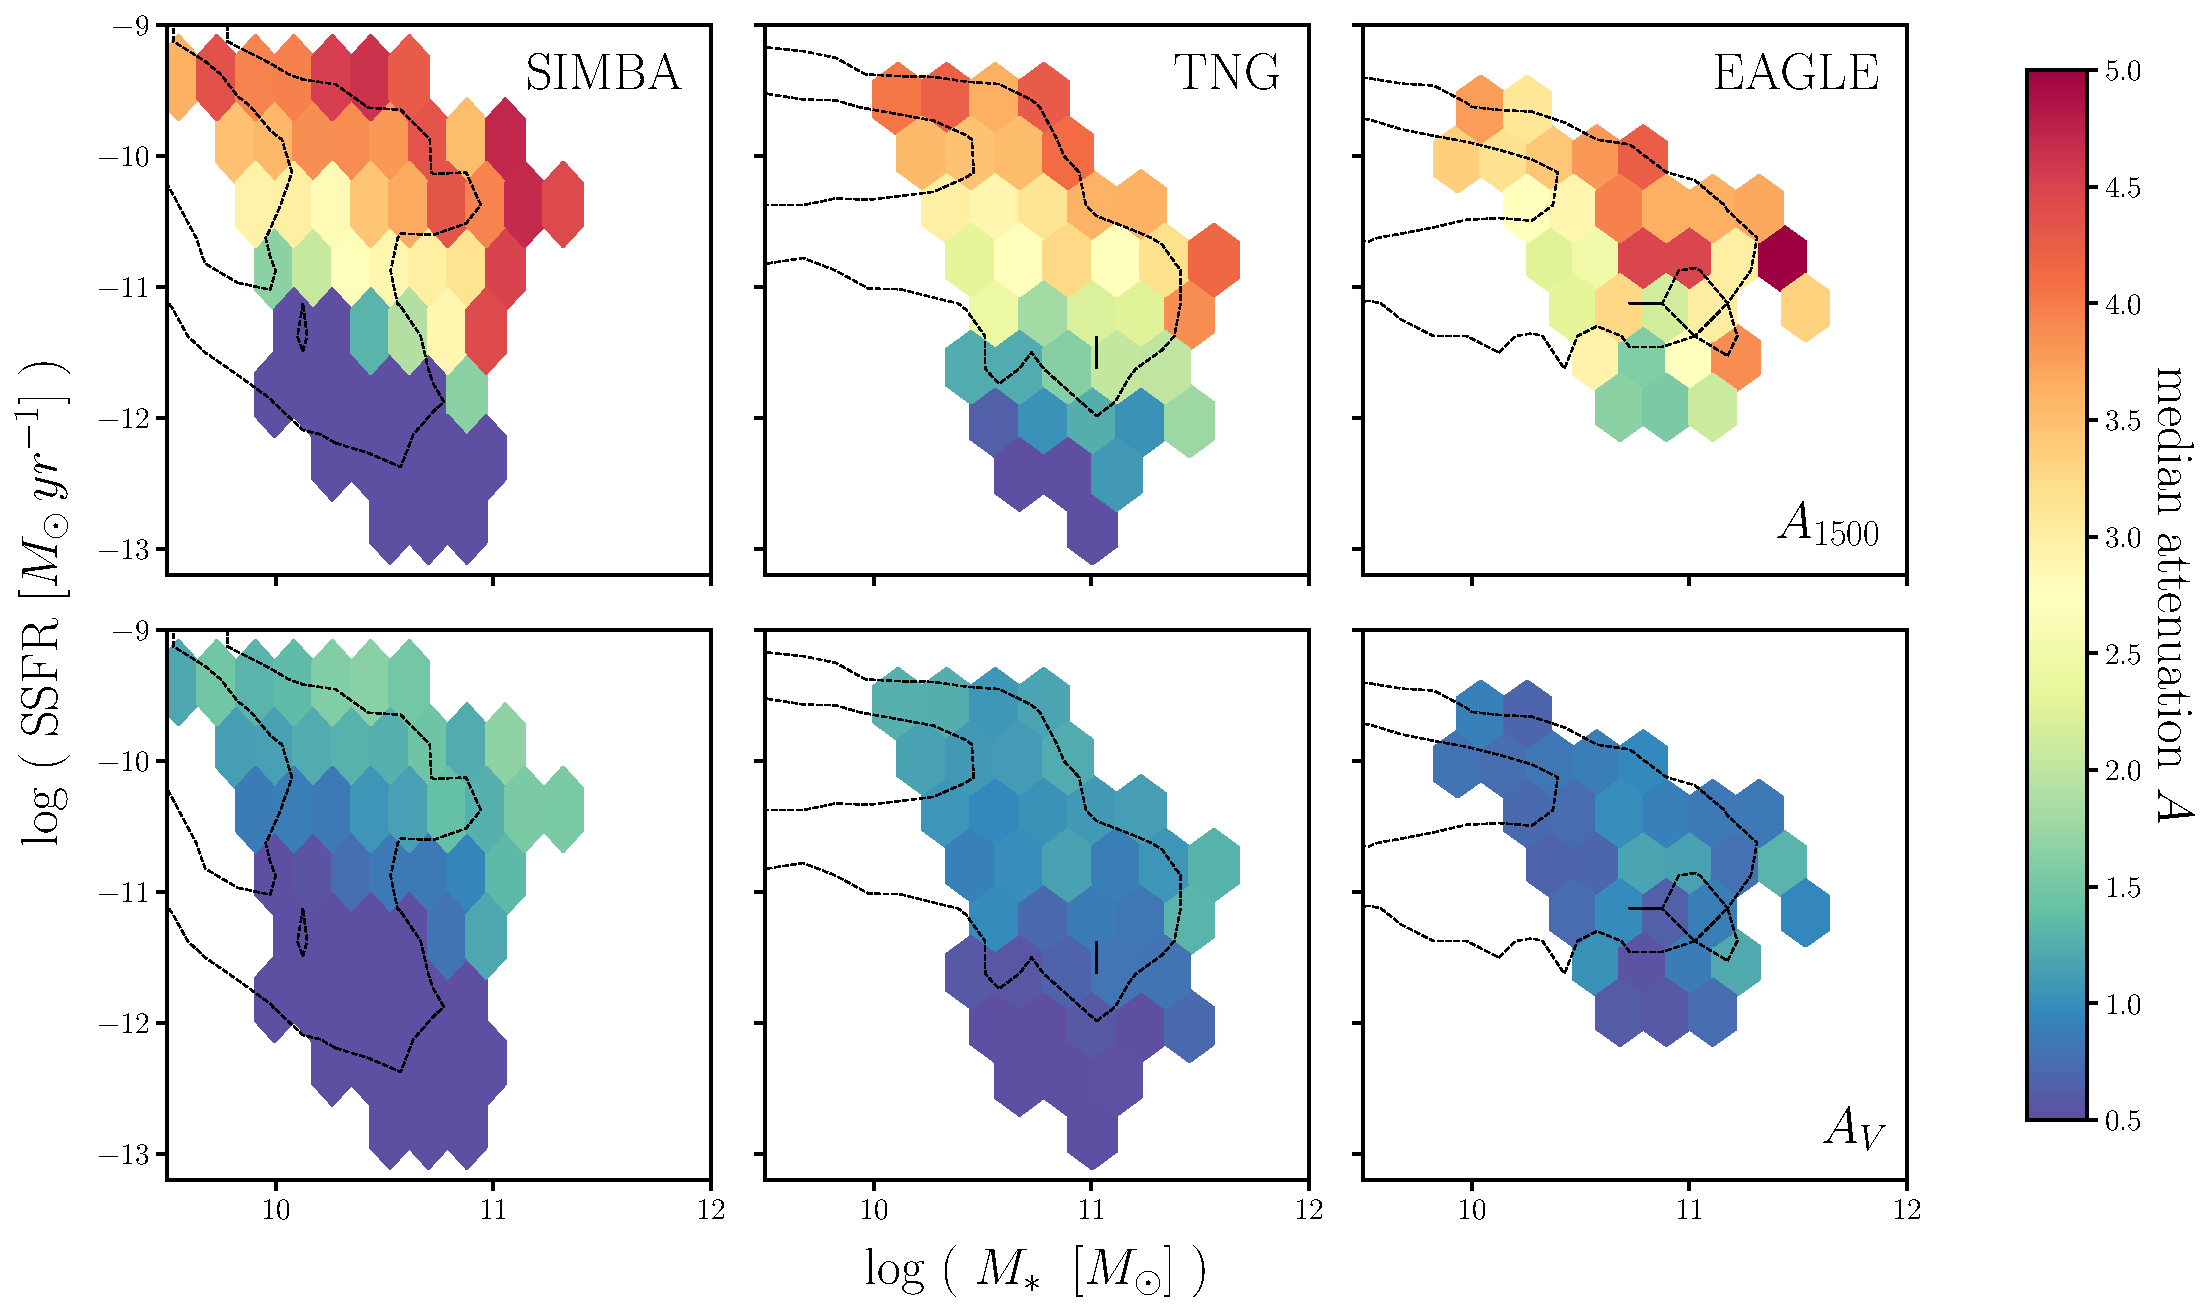
\includegraphics[width=0.9\textwidth]{figs/abc_av_mssfr.pdf}
    \caption{\label{fig:avmsfr}
        $M_*$ and $\ssfr$ dependence of dust attenuation at $1500 \AA$
        ($A_{1500}$; top) and at $5500\AA$ ($A_{V}$ bottom) predicted by the
        \eda~for SIMBA(left), TNG (center), and EAGLE (right). The colormap in each hexbin 
        represents the median attenuation for all simulated galaxies in the
        bin (right color bar). We only include bins with more than 10 galaxies.
        For reference, we include in each panel the $M_*-\ssfr$ relation of
        all galaxies from the simulations (black dashed).
        Overall, simulated galaxies with higher $M_*$ have higher dust
        attenuation at constant SSFR --- consistent with the literature.
        Furthermore, since previous works have primarily focused on star-forming
        galaxies, the \eda~provides new insight into the $\ssfr$ dependence of
        dust attenuation: simulated galaxies with higher $\ssfr$ have steeper
        attenuation curves. 
    }
\end{center}
\end{figure}

\subsection{The Galaxy -- Dust Connection}  
In the previous section, we presented the attenuation curves predicted by
the \eda~for quiescent galaxies. 
By comparing them to the attenuation curves of star-forming galaxies, we
found significant $\ssfr$ dependence in dust attenuation: quiescent galaxies
have attenuation curves with shallower slopes and lower amplitude than
star-forming galaxies. 
In this section, we examine the connection between dust attenuation and galaxy
properties in more detail. 
First, we examine the galaxy-dust connection using the $M_*$ and $\ssfr$
dependent parameterization of our
\eda~prescription (Eqs~\ref{eq:tauv} and~\ref{eq:delta}).
In Table~\ref{tab:posterior}, we list the median values and the 68\%
confidence interval of the inferred \eda~parameter posteriors for the 
three simulations. 
In addition to the $\ssfr$ dependence, we also find
significant $M_*$ dependence in $\tau_V$: $m_{\tau,M_*} > 0$.
$V$-band dust attenuation is higher for more massive galaxies.  
There is, however, little $M_*$ dependence in the slope of the dust
attenuation.

%%%%%%%%%%%%%%%%%%%%%%%%%%%%%%%%%%%%%%%%%%
% table of free parameters
%%%%%%%%%%%%%%%%%%%%%%%%%%%%%%%%%%%%%%%%%%
\begin{table}
    \caption{Inferred the Empirical Dust Attenuation Model Parameters}
    \begin{tabular}{lcccccc} \toprule
        & $m_{\tau,M_*}$ & $m_{\tau,\ssfr}$ & $c_\tau$ & $m_{\delta,M_*}$ & $m_{\delta,\ssfr}$ & $c_\delta$ \\[3pt] \hline\hline
        SIMBA   & $1.27\substack{+0.46\\-0.46}$ &
        $1.28\substack{+0.24\\-0.23}$ & $1.58\substack{+0.12\\-0.12}$ &
        $0.07 \substack{+0.12\\-0.11}$ & $0.13 \substack{+0.10\\-0.10}$ &
        $-0.18\substack{+0.04\\-0.04}$ \\
        TNG     & $0.57\substack{+0.44\\-0.53}$ &
        $0.62\substack{+0.21\\-0.20}$ & $1.34\substack{+0.19\\-0.21}$ &
        $-0.18\substack{+0.20\\-0.19}$ & $-0.19\substack{+0.15\\-0.16}$ &
        $-0.07\substack{+0.08\\-0.08}$ \\
        EAGLE   & $0.59\substack{+0.33\\-0.33}$ &
        $0.18\substack{+0.20\\-0.17}$ & $0.81\substack{+0.14\\-0.15}$ &
        $-0.13\substack{+0.17\\-0.18}$ & $-0.22\substack{+0.14\\-0.14}$ &
        $-0.34\substack{+0.08\\-0.08}$\\
        \hline
    \end{tabular} \label{tab:posterior}
\end{table}

We take a closer look at the $M_*$ and $\ssfr$ dependence of the attenuation
curve in Figure~\ref{fig:avmsfr}, where we present dust attenuation at
$1500\AA$ ($A_{1500}$; top) and $5500\AA$
($A_V$; bottom) as a function of $\log M_*$ and $\log \ssfr$ predicted by the
\eda~for SIMBA (left), TNG (center) and EAGLE (right). 
For each hexbin, the colormap represents the median attenuation for all
simulated galaxies in the bin. 
We only include bins with more than 10 galaxies. 
We include, for reference, the $M_* - \ssfr$ relation of all galaxies in the
simulations in black dashed contours, which mark the 68 and 95 percentiles.
We do not include a direct comparison with $A_{1500}$ and $A_V$ measured
from observations because there are large variations between different
measurements (Appendix~\ref{sec:slab}, see also Figure~\ref{fig:av_obs}).  

In each panel, we find that SIMBA, TNG, and EAGLE galaxies with higher
$M_*$ have higher dust attenuation at constant SSFR --- consistent with the literature.
\cite{burgarella2005}, for instance, found significant positive $M_*$
dependence in $FUV$ attenuation in NUV-selected and FIR-selected samples. 
\cite{garn2010} and \cite{battisti2016} also find higher attenuation in
more massive SDSS star-forming galaxies. 
Most recently, \cite{salim2018} find higher $V$ and $FUV$ attenuation for
more massive star-forming galaxies in GSWLC2. 
For the $\ssfr$ dependence, we find that galaxies with higher $\ssfr$ have
higher $A_{1500}$ (top) and $A_V$ (bottom) as well as steeper slopes. 
The $\ssfr$ dependence is not as prominent in EAGLE (see also
Table~\ref{tab:posterior}), which has a narrower $\ssfr$ distribution than
SIMBA and TNG with no starburst galaxies or quiescent galaxies with $\ssfr <
10^{-12}yr^{-1}$. 
EAGLE, therefore, has fewer intrinsically luminous star-forming galaxies
or UV red galaxies (Figure~\ref{fig:obs}) and a narrower intrinsic $\gr$
and $\fnuv$ color distributions. 
To reproduce observations, it requires an overall attenuation and reddenning
without a significant $\ssfr$ dependence. 
Nevertheless, in all simulations, star-forming galaxies have slopes that
are consistent with observations (Section~\ref{sec:reproduce}) while
quiescent galaxies with the lowest $\ssfr$ have nearly flat attenuation
curves. 
Since observations have only focused on star-forming galaxies due to the
difficulty in measuring dust attenuation in quiescent galaxies, the
\eda~predictions provide new insight into the $\ssfr$ dependence of dust
attenuation. 
In summary, we find that \emph{SIMBA, TNG, and EAGLE galaxies with higher
$M_*$ require overall higher dust attenuation and galaxies with higher
$\ssfr$ require steeper attenuation curves}.
